% \documentclass[12pt]{article}
\documentclass[12pt,fleqn]{article}
\usepackage[utf8]{inputenc}
\usepackage[russian]{babel}
\usepackage{graphicx}
\usepackage{array}
\usepackage[a4paper, left=1cm, right=1cm, top=1.27cm, bottom=1.27cm]{geometry}
\usepackage{setspace}
\usepackage{tabularx}
\usepackage{makecell}
\usepackage{longtable}
\usepackage{multirow}
\usepackage{caption}
\usepackage{amsmath}
\usepackage{amssymb}
\usepackage{ragged2e}
\onehalfspacing


\begin{document}


\begin{table}[h]
    \centering
    \renewcommand{\arraystretch}{1.5}
    \begin{tabular}{m{11cm}m{6cm}}
        \begin{center}
            \textbf{Университет ИТМО}\\
            \textbf{Физико-технический мегафакультет}\\
            \textbf{Физический факультет}
        \end{center} 
        & 
        \begin{center}
            
\includegraphics[height=1.3cm]{logo.jpg}
        \end{center} \\
    \end{tabular}
\end{table}

\noindent\makebox[\linewidth]{\rule{\textwidth}{2pt}}

\vspace{10pt}

\begin{table}[h]
    \centering
    \renewcommand{\arraystretch}{1.7}
    \begin{tabular}{p{4cm}p{4cm}p{8cm}}
        Группа N3250 & & К работе допущен \underline{\hspace{4cm}} \\
        Студенты & \hfill \multirow[0pt]{3}{*}{\makecell[c]{Пахомов В.Ю \\ Булин М.М \\ Рулев М.Ю}}  & Работа выполнена \underline{\hspace{4cm}} \\
        & & \\
        & & \\
        \multicolumn{2}{l}{Преподаватель Рудель А.Е}  & Отчет принят \underline{\hspace{5cm}} \\
    \end{tabular}
\end{table}

\begin{center}
    \fontsize{20pt}{21.5pt} \selectfont
    \textbf{Рабочий протокол и отчет по} \\
    \textbf{лабораторной работе № 3.07}
\end{center}

\noindent\makebox[\linewidth]{\rule{\textwidth}{1pt}}
\noindent\makebox[\linewidth]{\rule{\textwidth}{1pt}}

\begin{justify}
    \textbf{1. Цель работы} \\
    Изучить свойства ферромагнетика. \\
\end{justify}

\begin{justify}
    \textbf{2. Задачи, решаемые при выполнении работы} \\
    1) Измерение зависимости магнитной индукции в ферромагнетике от напряженности магнитного поля $ B = B(H) $. \\
    2) Определение по предельной петле гистерезиса индукции насыщения, остаточной индукции и коэрцитивной силы. \\
    3) Получение зависимости магнитной проницаемости от напряженности магнитного поля $ \mu = \mu(H) $ и оценка максимального значения величины магнитной проницаемости \\
    4) Расчет мощности потерь энергии в ферромагнетике в процессе его перемагничивания. \\
\end{justify}

\begin{justify}
    \textbf{3. Объект исследования} \\
    Ферромагнетик – сердечник (магнитопровод) трансформатора прямоугольной формы с прямоугольным поперечным сечением. \\
\end{justify}

\begin{justify}
    \textbf{4. Метод экспериментального исследования} \\
    Магнитные свойства ферромагнетика изучаются по петле гистерезиса, наблюдаемой на осциллографе. \\
\end{justify}

\begin{justify}
    \textbf{5. Рабочие формулы и исходные данные} \\
    $ H = \alpha K_x x, \quad \alpha = \frac{N_1}{L R_1} $ \\
    $ B = \beta K_y y, \quad \beta = \frac{R_2 C_1}{N_2 S} $ \\
    $ \mu = \frac{B}{\mu_0 H} $ \\
    $ P = \chi \cdot S_{\text{ПГ}}, \quad \chi = K_x K_y \frac{N_1 R_2 C_1}{N_2 R_1} f $ \\
\end{justify}


\begin{flushleft}
    \textbf{6. Измерительные приборы} \\
    \begin{table}[h]
    \centering
    \renewcommand{\arraystretch}{1.5}
    \begin{tabular}{|c|c|c|c|c|}
        \hline
        № п/п & Наименование & Тип прибора & Используемый диапазон & Погрешность прибора\\
        \hline
        1 & С3-РМ01 & Стенд & 0-20 В & 0.1 В \\
        \hline
        2 & АКИП-3409/2 & Генератор сигналов & 20-40 Гц & 0.1 Гц \\
        \hline
        3 & GDS-71102В & Осцилограф & 0-20 В & 0.1В \\
        \hline
    \end{tabular}
    \end{table}
\end{flushleft}


\begin{flushleft}
    \textbf{7. Схема установки} \\
    \begin{figure}[h!]
        \centering
        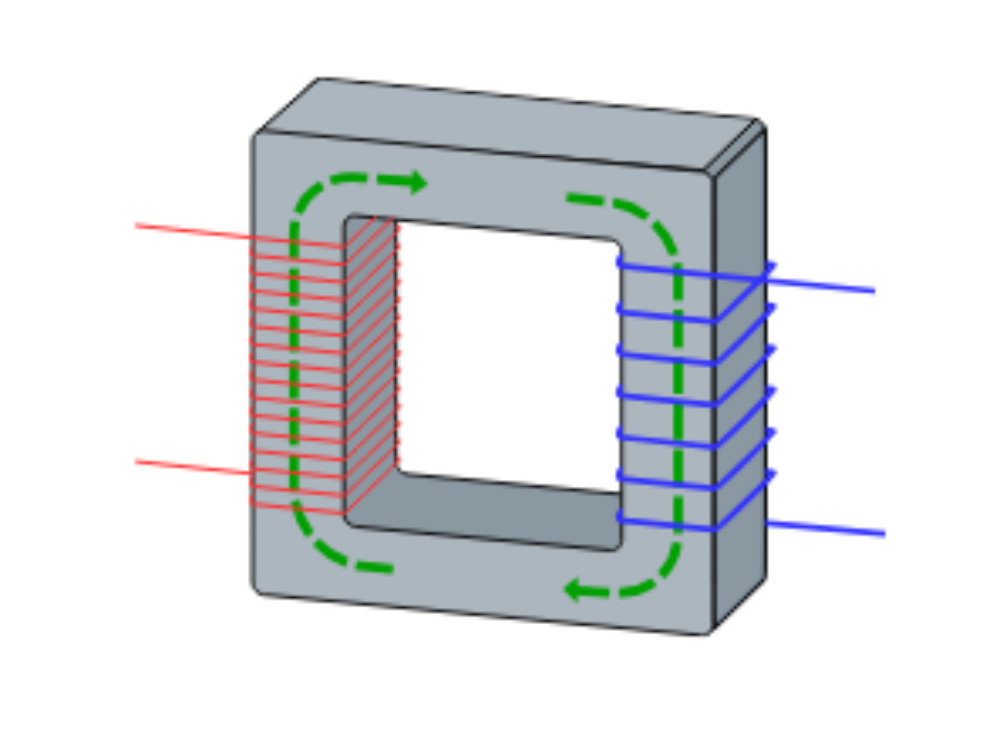
\includegraphics[height=10cm]{schema1.png}
        \caption{Магнитопровод (сердечник) трансформатора}
    \end{figure}
    \begin{figure}[h!]
        \centering
        
\includegraphics[height=10cm]{schema2.png}
        \caption{Принципиальная электрическая схема установки}
    \end{figure}
\end{flushleft}


\newpage


\begin{flushleft}
    \textbf{8. Результаты прямых измерений и их обработки} \\

    \begin{table}[h!]
    \centering
    \caption{Результаты измерений и расчётов магнитной индукции и проницаемости}
    \begin{tabular}{|c|c|c|c|c|c|c|c|}
    \hline
    $U$, В & $X$, дел & $K_x$, В/дел & $H$, А/м & $Y$, дел & $K_y$, В/дел & $B$, Тл & $\mu$ \\ \hline
    20 & 1.3 & 0.1 & 40.8 & 1.6 & 0.05 & 0.285 & 5554 \\ \hline
    19 & 1.2 & 0.1 & 37.9 & 1.5 & 0.05 & 0.267 & 5610 \\ \hline
    18 & 1.1 & 0.1 & 34.6 & 1.4 & 0.05 & 0.249 & 5711 \\ \hline
    17 & 1.1 & 0.1 & 34.6 & 1.3 & 0.05 & 0.231 & 5335 \\ \hline
    16 & 1.0 & 0.1 & 31.4 & 1.2 & 0.05 & 0.214 & 5413 \\ \hline
    15 & 0.9 & 0.1 & 28.5 & 1.1 & 0.05 & 0.196 & 5485 \\ \hline
    14 & 0.9 & 0.1 & 28.5 & 1.1 & 0.05 & 0.196 & 5485 \\ \hline
    13 & 0.8 & 0.1 & 25.2 & 1.0 & 0.05 & 0.178 & 5602 \\ \hline
    12 & 0.8 & 0.1 & 25.2 & 1.0 & 0.05 & 0.178 & 5602 \\ \hline
    11 & 0.7 & 0.1 & 21.8 & 0.9 & 0.05 & 0.160 & 5831 \\ \hline
    10 & 0.6 & 0.1 & 18.9 & 0.8 & 0.05 & 0.143 & 6010 \\ \hline
    9  & 1.3 & 0.05 & 40.8 & 2.0 & 0.02 & 0.356 & 6934 \\ \hline
    8  & 1.2 & 0.05 & 37.9 & 1.8 & 0.02 & 0.321 & 6746 \\ \hline
    7  & 1.1 & 0.05 & 34.6 & 1.6 & 0.02 & 0.285 & 6550 \\ \hline
    6  & 1.0 & 0.05 & 31.4 & 1.2 & 0.02 & 0.214 & 5413 \\ \hline
    5  & 0.9 & 0.05 & 28.5 & 1.0 & 0.02 & 0.178 & 4983 \\ \hline
    \end{tabular}
    \end{table}


\end{flushleft}


\newpage


\begin{justify}
    \textbf{9. Расчет результатов косвенных измерений (таблицы, примеры расчетов).} \\
    $ \alpha = \frac{N_1}{LR_1} = \frac{1665}{0.078 \cdot 68} = 313.91 \; \frac{1}{\text{м} \cdot \text{Ом}} $ \\
    $ \beta = \frac{R_2C_1}{N_2S} = \frac{47000 \cdot 0.47 \cdot 10^{-6}}{970 \cdot 0.64 \cdot 10^{-4}} = 0.356 \; \frac{\text{Ом} \cdot \text{Ф}}{\text{м}} $ \\
    $ H_c = \alpha K_x x = 313.91 \cdot 0.1 \cdot 1.1 = 34.53 \; \text{А/м}$ \\
    $ B_r = \beta K_y y = 3.56 \cdot 0.05 \cdot 1.2 = 0.21 \; \text{Тл} $ \\
    \begin{table}[h]
    \centering
    \caption{}
    \renewcommand{\arraystretch}{1.5}
    \begin{tabular}{|c|c|c|c|}
        \hline
        $X_c$, дел. & $Y_r$, дел. & $H_c$, A/м & $B_r$, Тл \\
        \hline
        1.1 & 1.2 & 34.53 & 0.21 \\
        \hline
    \end{tabular}
    \end{table}
    $ H_m = \alpha K_x x = 313.91 \cdot 0.1 \cdot 1.6 = 50.23 \; \text{А/м}$ \\
    $ B_m = \beta K_y y = 3.56 \cdot 0.05 \cdot 1.4 = 0.25 \; \text{Тл} $ \\
    $ \mu_0 = 4\pi \cdot 10^{-7}$ Гн/м\\
    $ \mu_m = \frac{B}{\mu_0 H} = \frac{0.25}{4\pi \cdot 10^{-7} \cdot 50.23} = 3948 $ Гн/м \\
    \begin{table}[h]
    \centering
    \caption{}
    \renewcommand{\arraystretch}{1.5}
    \begin{tabular}{|c|c|c|c|c|}
        \hline
        $X_m$, дел. & $Y_m$, дел. & $H_m$, A/м & $B_m$, Тл & $ \mu_m $  \\
        \hline
        1.6 & 1.4 & 50.23 & 0.25 & 3948 \\
        \hline
    \end{tabular}
    \end{table}

    Для первой строки таблицы: \\
    $ H = \alpha K_x x, \quad \alpha = \frac{N_1}{L R_1} = 3.13 \cdot 0.1 \cdot 1.3 = 40.8 $ А/м\\
    $ B = \beta K_y y, \quad \beta = \frac{R_2 C_1}{N_2 S} = 3.56 \cdot 0.05 \cdot 1.6 = 0.285 $ \\
    $ \mu = \frac{0.285}{4\pi \cdot 10^{-7} \cdot 40.8} = 5554 $ Гн/м \\
    $ \mu_{max} = 6934 $ Гн/м \\
    $ \chi = K_x K_y \frac{N_1 R_2 C_1}{N_2 R_1} f = \frac{0.1 \cdot 0.05}{1665 \cdot 470000 \cdot 0.00000047} \cdot \frac{970}{68} = 0.058 \; \frac{\text{Вт}}{\text{дел}^2} $ \\
    $ P = \chi \cdot S_{\text{ПГ}} = 0.0058 \cdot 7 = 0.0406 \; \text{Вт} $ \\


\end{justify}

\begin{justify}
    \textbf{10. Расчет погрешностей измерений (для прямых и косвенных измерений)} \\
    Коэрцитивная сила (Hc): \\
        \[ \varepsilon_{H_c} = \sqrt{\left(\frac{\Delta K_z}{K_z}\right)^2 + \left(\frac{\Delta x_c}{x_c}\right)^2} \]
        \[ H_c = 34.5 \pm 3.3~\text{А/м} \]
        Относительная погрешность: $\approx 9.6\%$ \\
    Остаточная индукция (Br): \\ 
        \[\varepsilon_{B_r} =  \sqrt{\left(\frac{\Delta K_y}{K_y}\right)^2 + \left(\frac{\Delta y_r}{y_r}\right)^2}\]
        \[ B_r = 0.21 \pm 0.02~\text{Тл} \]
        Относительная погрешность: $\approx 8.9\%$ \\
    Максимальная магнитная проницаемость ($\mu_{\max}$): \\ 
        \[ \varepsilon_\mu = \sqrt{\varepsilon_B^2 + \varepsilon_H^2} \]
        \[ \mu_{\max} = 6930 \pm 700 \]
        Относительная погрешность: $\approx 10.1\%$ \\
    Мощность потерь на перемагничивание (P): \\ 
        \[ \varepsilon_P = \sqrt{\varepsilon_x^2 + \varepsilon_S^2} \]
        (где $\varepsilon_S$ — погрешность определения площади, принятая 10\%)
        \[ P = 0.041 \pm 0.004~\text{Вт} \]
        Относительная погрешность: $\approx 10.9\%$ \\
\end{justify}


\newpage


\begin{justify}
    \textbf{11. Графики (перечень графиков, которые составляют Приложение 2)} \\
    \begin{figure}[h!]
    \centering
    
\includegraphics[height=10cm]{graphic1.png} \\
    \caption{График зависимости $ B_m = B_m(H_m) $ }
    \end{figure}

    \begin{figure}[h!]
    \centering
    
\includegraphics[height=10cm]{graphic2.png} \\
    \caption{График зависимости $ \mu = \mu(H_m) $ }
    \end{figure}
\end{justify}


\begin{justify}
    \textbf{12. Окончательные результаты} \\
    Коэрцитивная сила: $ H_c = 34.53 $ А/м \\
    Остаточная индукция: $ B_r = 0.21 $ Тл \\
    Магнитная проницаемость в состоянии насыщения: \\
    $ \mu_m = 3948 $ Гн/м \\
    Мощность потерь на перемагничивание ферромагнетика: \\
    $ P = 0.0406 $ мВт \\
    Максимальное значения проницаемости и напряжённость поля, при которой она наблюдается: \\
    $ \mu_{max} = 6934 $ Гн/м \\ 
\end{justify}

\begin{justify}
\textbf{13. Выводы и анализ результатов работы} \\
В ходе выполнения лабораторной работы были экспериментально исследованы основные 
магнитные характеристики ферромагнитного сердечника трансформатора. 
По полученной петле гистерезиса и зависимости магнитной индукции от 
напряжённости магнитного поля были определены следующие величины:

\begin{itemize}
    \item коэрцитивная сила: $ H_c = 34.5 \, \text{А/м} $;
    \item остаточная индукция: $ B_r = 0.21 \, \text{Тл} $;
    \item максимальная магнитная проницаемость: $ \mu_{\max} \approx 6.9 \cdot 10^{3} $;
    \item магнитная проницаемость в состоянии насыщения: $ \mu_m \approx 3.9 \cdot 10^{3} $;
    \item мощность потерь при перемагничивании: $ P \approx 0.041 \, \text{Вт} $.
\end{itemize}

Полученные результаты соответствуют характерным значениям для 
ферромагнитных материалов, обладающих заметной шириной петли гистерезиса. 
По графику $\mu(H)$ прослеживается рост магнитной проницаемости в области 
малых полей и её последующее снижение при приближении к насыщению, 
что согласуется с теоретическими ожиданиями.

Эксперимент подтвердил наличие магнитного гистерезиса и позволил 
оценить энергозатраты на перемагничивание исследуемого сердечника. 
В целом полученные данные демонстрируют хорошее соответствие 
теоретическим моделям ферромагнетиков и позволяют сделать вывод 
о корректности проведённых измерений.
\end{justify}


\begin{justify}
    \textbf{14. Дополнительные задания} \\
\end{justify}

\begin{justify}
    \textbf{15. Выполнение дополнительных заданий} \\
\end{justify}

\begin{justify}
    \textbf{16. Замечания преподавателя (исправления, вызванные замечаниями преподавателя, также помещают в этот пункт)} \\
\end{justify}

\end{document}
